\begin{frame}{Test bench}
	\only<1>{El sistema fue simulado con el objetivo de corroborar el correcto funcionamiento del sistema, cómo así también detectar fallas en la descripción realizada y obtener una forma de depuración de lo realizado.}
\end{frame}
\begin{frame}{Test bench - Top}
	\only<1>{
		\centering
		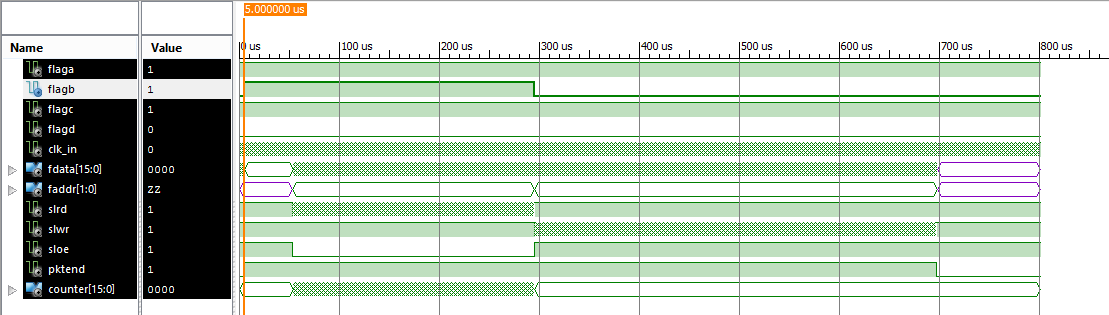
\includegraphics[width=\textwidth]{tb_top_ov}\\
		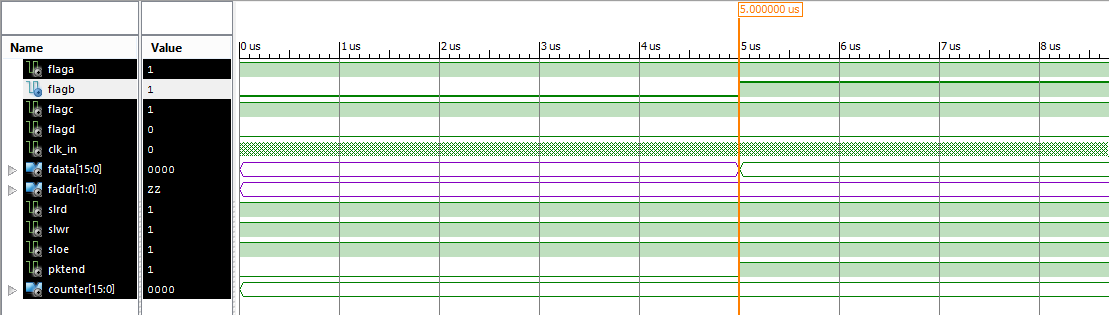
\includegraphics[width=\textwidth]{tb_top_rst}}
\end{frame}
\begin{frame}{Test bench - Lectura de la interfaz}
	\only<1>{
		\centering
		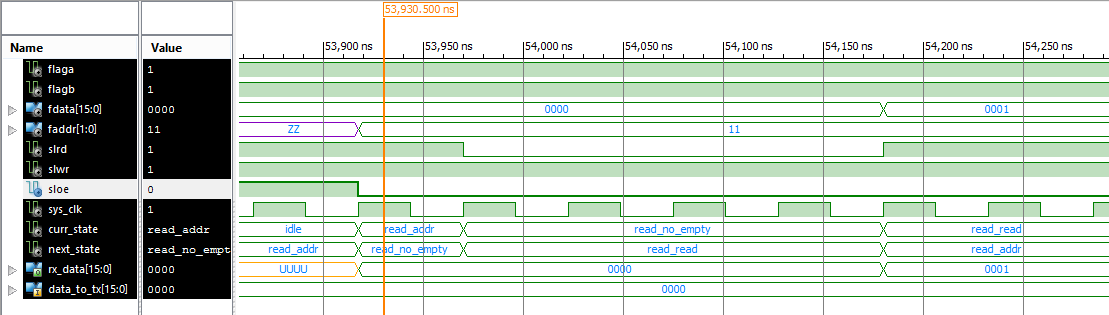
\includegraphics[width=\textwidth]{tb_if_rd_mef}\\
		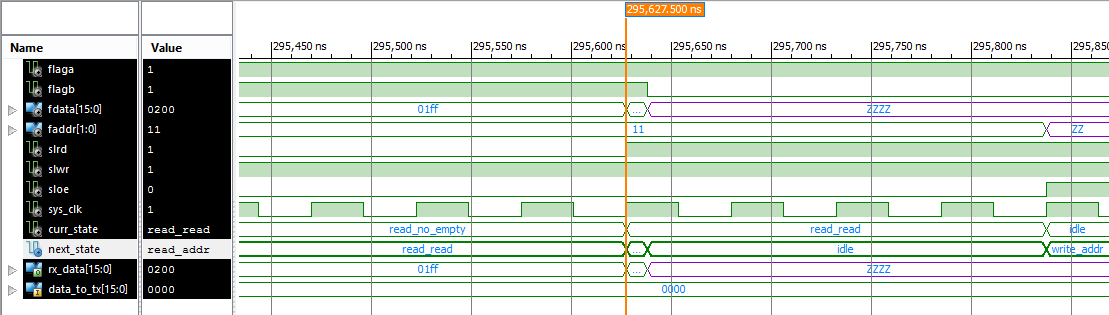
\includegraphics[width=\textwidth]{tb_if_rd_end}
		}
\end{frame}
\begin{frame}{Test bench - Escritura en la interfaz}
	\only<1>{
		\centering
		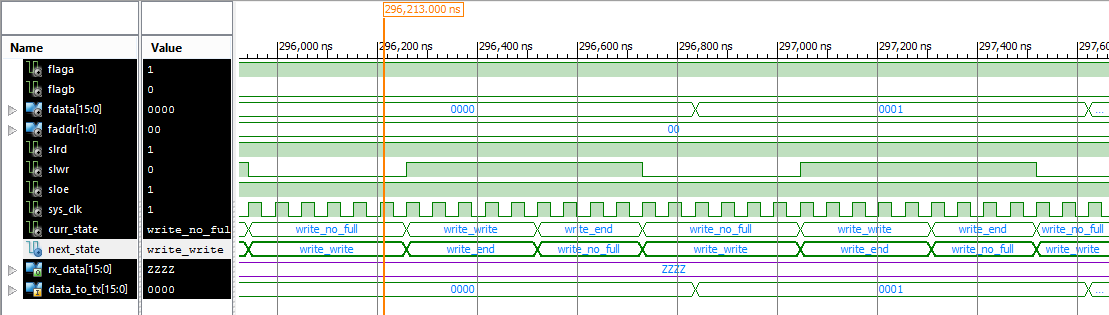
\includegraphics[width=\textwidth]{tb_if_wr_mef}\\
		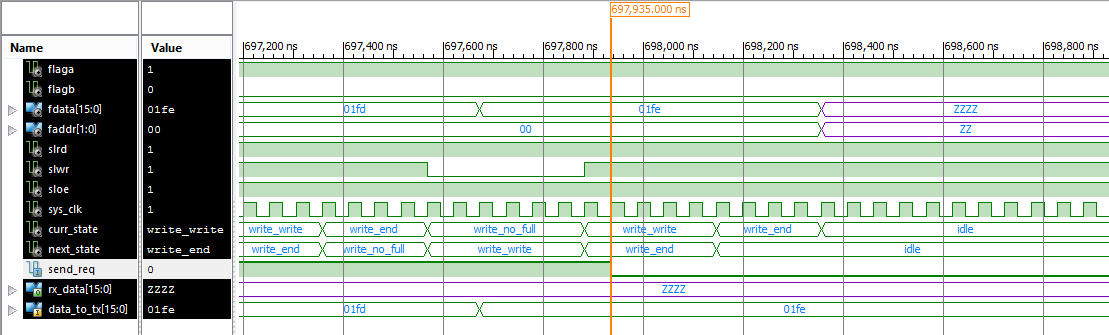
\includegraphics[width=\textwidth]{tb_if_wr_end}}
	\only<2>{
		\centering
		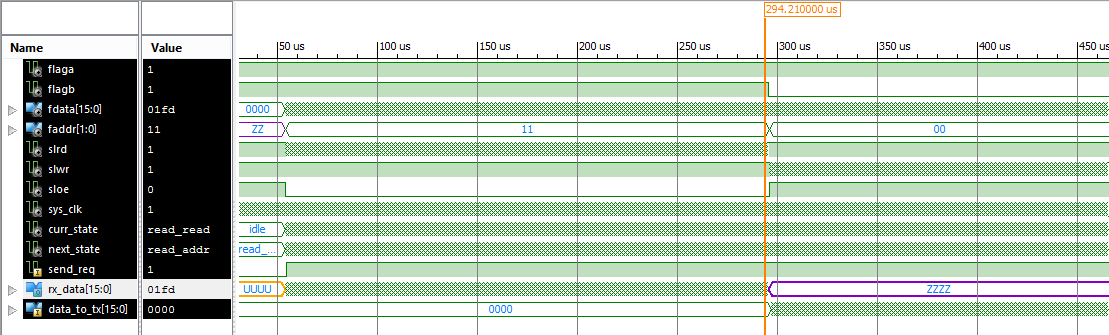
\includegraphics[width=\textwidth]{tb_if_snd}\\
		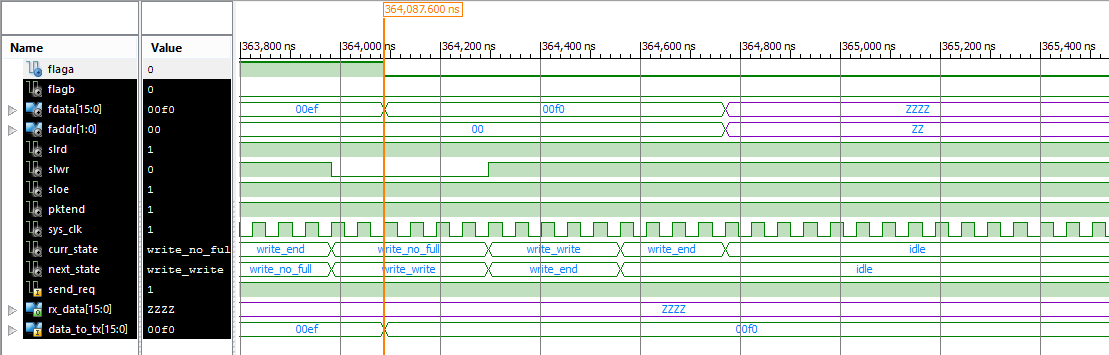
\includegraphics[width=\textwidth]{tb_if_fflag_end}}
\end{frame}
